\documentclass[master=ucll,dutch,twoside]{ucllfilip}
%\documentclass[master=bin,masteroption=eg]{kulemt}
%master is hetgene dat gedefinieerd staat in de .cfg file
%masteroption is hetgene bij ELT gedeelte staat als optie
%and command is voor een 2de lijn bij te voegen
\setup{
	title={Samenvatting Distributed Applications},
  author={Filip Vanden Eynde \and R0363898 \and 3TX/1},
  promotor={Professor Kasper Cools}}



% De volgende \ setup mag verwijderd worden als geen fiche gewenst is.
\setup{filingcard,
  translatedtitle={Portfolio money management},
translatedtitle={},
  udc=621.3,
  keywords={beleggen anders bekeken, ucll, portfolio},
  shortabstract={Hier komt een heel bondig abstract van hooguit 500
    woorden. \LaTeX\ commando's mogen hier gebruikt worden. Blanco lijnen
    (of het commando \texttt{\string\pa r}) zijn wel niet toegelaten!
   \endgraf \lipsum[2]}}

% Verwijder de "%" op de volgende lijn als je de kaft wil afdrukken
%\setup{coverpageonly}
\write18{pdflatex masterproefcoverpage -aux-directory=outputfoldercoverpage}
%\write18{pdflatex masterproefcoverpage}

% Verwijder de "%" op de volgende lijn als je enkel de eerste pagina's wil
% afdrukken en de rest bv. via Word aanmaken.
%\setup{frontpagesonly}

\newcommand{\kleurlinkstableofcontents}{blue}

% Kies de fonts voor de gewone tekst, bv. Latin Modern
%\setup{font=palatino}

\setup{font=utopia}

\setup{inputenc=utf8}

\usepackage{ifthen}
\newboolean{pdfoutput}
\setboolean{pdfoutput}{true}
%\setboolean{pdfoutput}{false}

% Hier kun je dan nog andere pakketten laden of eigen definities voorzien

\usepackage{ucllfilip}
\chapterstyle{ucllfilipman}
\ucllfilipmanToC{}

\usepackage{minted}

\usepackage{booktabs}
\usepackage{colortbl}
\usepackage[table,dvipsnames]{xcolor}
\usepackage{subcaption}

%\usepackage{geometry}
%\usepackage{pdflscape}
%for bibliography
\usepackage[backend=biber,
%style=alphabetic,
style=numeric,
%style=ieee,
%style=ieee-alphabetic,
citestyle=numeric,
%refsection=chapter,
refsegment=chapter,
defernumbers=true,
%sorting=ynt,
sorting=nty
]{biblatex}
%\addbibresource{referenties.bib}

\addbibresource{resources.bib} %Imports bibliography file
\addbibresource{chapter1.bib}
%\addbibresource{chapter2.bib}
%\addbibresource{chapter3.bib}
%\addbibresource{chapter4.bib}

%\defbibheading{subbibliography}{%
%	\section*{References for Chapter \ref{refsection:
%			,→ \therefsection}}}


\defbibheading{bibliography}[\bibname]{%
	\section{#1}%
	\markboth{#1}{#1}}


%indexes
%voor indexen te maken
\usepackage{imakeidx}
\makeindex[
%columns=3, % geeft layout van 3 kolommen
title=Alphabetical Index, % verandert de default title = index
intoc] % voegt de indexpagina aan de inhoudsopgave toe

\usepackage{import}
\usepackage{enumitem}
\usepackage{pdfpages}
%\usepackage{todo}
\usepackage{todonotes}

%provides the multicols environment which typesets text into multiple columns.
\usepackage{multicol}
\usepackage[official]{eurosym}

%-------------------------------------------------------------------------------------------------------------------------
% pas plaats voor en na headings aan gebruikmakend van package titlesec
%-------------------------------------------------------------------------------------------------------------------------

\usepackage{titlesec}
%\titlespacing\section{0pt}{12pt plus 4pt minus 2pt}{0pt plus 2pt minus 2pt}
%\titlespacing\subsection{0pt}{12pt plus 4pt minus 2pt}{0pt plus 2pt minus 2pt}

%------------------------------------------------------------------------

% Define a set of colours for syntax highlighting

\definecolor{MyColor1}{rgb}{0.2,0.4,0.6} %mix personal color
\definecolor{azure(colorwheel)}{rgb}{0.0, 0.5, 1.0}
\newcommand{\textb}{\color{Black} \usefont{OT1}{lmss}{m}{n}}
\newcommand{\blue}{\color{MyColor1} \usefont{OT1}{lmss}{m}{n}}
\newcommand{\blueb}{\color{MyColor1} \usefont{OT1}{lmss}{b}{n}}
\definecolor{purpleexcel}{rgb}{0.4392156862745,0.18823529,0.62745098039}
\definecolor{dkgreen}{rgb}{0,.6,0}%
\definecolor{dkblue}{rgb}{0,0,.6}%
\definecolor{dkyellow}{cmyk}{0,0,.8,.3}%
\definecolor{lightgray}{rgb}{0.95, 0.95, 0.95}%
\definecolor{darkgray}{rgb}{0.4, 0.4, 0.4}%
\definecolor{editorGray}{rgb}{0.95, 0.95, 0.95}%
\definecolor{editorOcher}{rgb}{1, 0.5, 0}%
\definecolor{editorGreen}{rgb}{0, 0.5, 0}%
\definecolor{orange}{rgb}{1,0.45,0.13}%
\definecolor{olive}{rgb}{0.17,0.59,0.20}%
\definecolor{brown}{rgb}{0.69,0.31,0.31}%
\definecolor{purple}{rgb}{0.38,0.18,0.81}%
\definecolor{lightblue}{rgb}{0.1,0.57,0.7}%
\definecolor{lightred}{rgb}{1,0.4,0.5}%
\definecolor{ChapBlue}{rgb}{0.00,0.65,0.65}

%hier komen alle commando's en constante variabelen voor in de opdracht te gebruiken.
\newcommand{\functiejob}{Softwareontwikkelaar}
\graphicspath{{images/}} % Set the default folder for images
%I usually write something like this, so the entry is hyperlinked for onscreen reading but there's also a footnote to the URL for paper output.
\newcommand\fnurl[2]{%
	\href{#2}{#1}\footnote{\url{#2}}%
}
%\setlist[itemize,1]{leftmargin=*,topsep=0pt}
%\setlist[enumerate,1]{leftmargin=*,topsep=0pt}
\setlist{nosep}
%\newcommand{\tabelgeometry}{%
%\newgeometry{total={7.7in, 9.5in},top=0.7in,bottom=0.7in}
%}

\renewcommand\mempostaddapppagetotochook{\cftinserthook{toc}{BREAK}}
\cftinsertcode{BREAK}{\changetocdepth{-10}}
\let\normalchangetocdepth\changetocdepth % needed for later

\makeatletter
\newcommand\appendixtableofcontents{
	\begingroup
	\let\changetocdepth\@gobble
	\normalchangetocdepth{-10}
	\cftinsertcode{BREAK}{\normalchangetocdepth{3}}
	\renewcommand\contentsname{Appendices overzicht}
	\tableofcontents*
	\endgroup
}
\makeatother


%\chapterstyle{BlueBox}



\ifthenelse {\boolean{pdfoutput}}
	{
	\usepackage[
	%hidelinks = true,
	pdfusetitle,colorlinks,urlcolor=magenta,linkcolor=\kleurlinkstableofcontents,
	plainpages=false,bookmarks=true,bookmarksnumbered,linktoc=all,pdffitwindow=true,
	pdftex,pdfauthor={\theauthor},pdftitle={\thetitle},pdfsubject={\thesubject},
	pdfkeywords={\thekeywords},pdfproducer={\theauthor},pdfcreator={\theauthor}
	]{hyperref}	
	}{
%\usepackage[
%hidelinks = true,
%pdfusetitle,colorlinks,urlcolor=magenta,linkcolor=\kleurlinkstableofcontents,
%plainpages=false,bookmarks=true,bookmarksnumbered,linktoc=all,pdffitwindow=true,
%pdftex,pdfauthor={\theauthor},pdftitle={\thetitle},pdfsubject={\thesubject},
%pdfkeywords={\thekeywords},pdfproducer={\theauthor},pdfcreator={\theauthor}
%]{hyperref}

%\usepackage{nohyperref}  % This makes hyperref commands do nothing without errors
%\usepackage{url}  % This makes \url work

\usepackage[draft]{hyperref}
}


\begin{comment}
% Tenslotte wordt hyperref gebruikt voor pdf bestanden.
% Dit mag verwijderd worden voor de af te drukken versie.
\usepackage[
%hidelinks = true,
pdfusetitle,
colorlinks,
urlcolor=magenta,
linkcolor=\kleurlinkstableofcontents,
%linkcolor=black, %Verander dit om de linkkleuren van de tableofcontents aan te passen
%colorlinks=false, %links krijgen kleuren of niet
plainpages=false,
bookmarks=true,
bookmarksnumbered,
linktoc=all, %maakt zowel de tekst als het paginanummer klikbaar en gelinkt
pdffitwindow=true,
pdftex,
%% PDF Author
pdfauthor={\theauthor},
%% PDF title
pdftitle={\thetitle},
%% PDF Subject
pdfsubject={\thesubject},
%% PDF Keywords
pdfkeywords={\thekeywords},
%% PDF producer
pdfproducer={\theauthor},
%% PDF Creator
pdfcreator={\theauthor}
]{hyperref}

\end{comment}



%%%%%%%
% Om wat tekst te genereren wordt hier het lipsum pakket gebruikt.
% Bij een echte masterproef heb je dit natuurlijk nooit nodig!
\IfFileExists{lipsum.sty}%
 {\usepackage{lipsum}\setlipsumdefault{11-13}}%
 {\newcommand{\lipsum}[1][11-13]{\par Hier komt wat tekst: lipsum ##1.\par}}
%%%%%%%




%\includeonly{hfdst-n}
\begin{document}


\begin{comment}
\begin{preface}
Graag bedank ik iedereen die mij hierbij ondersteund heeft, namelijk mijn professor, mijn vrienden en klasgenoten, alsook mijn familie.

%Dit is mijn dankwoord om iedereen te danken die mij bezig gehouden heeft. Hierbij dank ik mijn professor, mijn vrienden en mijn klasgenoten.  Ook mijn familie heeft mij erg gesteund natuurlijk.


\end{preface}
\end{comment}


\tableofcontents*
%\tableofcontents

\begin{comment}
\begin{abstract}	
	
  In dit \texttt{abstract} environment wordt een al dan niet uitgebreide
  samenvatting van het werk gegeven. De bedoeling is wel dat dit tot
  1~bladzijde beperkt blijft.

  \lipsum[1]

  \todo[inline]{Samenvatting schrijven}



\end{abstract}
\end{comment}

% Een lijst van figuren en tabellen is optioneel
%\listoffigures
%\listoftables
% Bij een beperkt aantal figuren en tabellen gebruik je liever het volgende:
\listoffiguresandtables
\todo[inline]{Nakijken of alle labels van figuren en tabellen uniek en duidelijk gedefinieerd zijn?}

\begin{comment}
% De lijst van symbolen is eveneens optioneel.
% Deze lijst moet wel manueel aangemaakt worden, bv. als volgt:
\chapter{Lijst van afkortingen en symbolen}
\section*{Afkortingen}
\begin{flushleft}
  \renewcommand{\arraystretch}{1.1}
  \begin{tabularx}{\textwidth}{@{}p{12mm}X@{}}
   %LoG   & Laplacian-of-Gaussian \\
   %MSE   & Mean Square error \\
   %PSNR  & Peak Signal-to-Noise ratio \\
  \end{tabularx}
\end{flushleft}
\section*{Symbolen}
\begin{flushleft}
  \renewcommand{\arraystretch}{1.1}
  \begin{tabularx}{\textwidth}{@{}p{12mm}X@{}}
    %42    & ``The Answer to the Ultimate Question of Life, the Universe,
    %        and Everything'' volgens de \cite{h2g2} \\
    %$c$   & Lichtsnelheid \\
    %$E$   & Energie \\
    %$m$   & Massa \\
    %$\pi$ & Het getal pi \\
  \end{tabularx}
\end{flushleft}
\end{comment}

\todo[inline]{Op het einde de list of todos verwijderen.}
\listoftodos

% Nu begint de eigenlijke tekst
\mainmatter

\clearforchapter
%\pagestyle{filip}

%\chapter{Financieel plan}
\label{financieelplan}

Uitleg: Omschrijf kort de functie die je zal uitoefenen. Bepaal het \textbf{loon} dat je daar zal krijgen als afgestudeerde bachelor student informatica. Wordt je loon
jaarlijks geïndexeerd? Verwacht je opslag na een aantal jaren?

In de lessen bespreken we hoe je een persoonlijk financieel plan schrijft. We starten met het
schrijven van je persoonlijke financieel plan (oefening 4.3). Je werkt dit verder uit, en steekt je
persoonlijk financieel plan in deel 1 van je portfolio.\newline\newline

Ik begin te werken in juli 2016 als \functiejob in een bedrijf.


Als je niet goed weet wat een masterproef is, kan je altijd Wikipedia\cite{Wikipedia} eens nakijken.

%\section{Lorem ipsum 4--5}
%\lipsum[1-2]

\newpage
\section{Budget\index{budget}}

Stel voor het eerste jaar een \textbf{budget} op. Gebruik het voorbeeld dat je kan vinden in het handboek beleggingsleer pagina 120. Bepaal zelf of je een vriend(in) hebt of dat je alleenstaand bent. Een aantal opmerkingen:
\begin{itemize}
	\item heb je een vriend(in), bespreek dan kort haar persoonlijke situatie (leeftijd,werk, loon,…).
	\item ga je nog thuis blijven wonen het eerste jaar of ga je een appartement of huis huren? Zoek dan zelf op websites een geschikte woning, en neem de
	huurprijs op in je budget.
	\item raam je inkomsten en uitgaven en vermeldt duidelijk je bronnen en de
	veronderstellingen die je inbouwt.
\end{itemize}

\subsection{Inkomsten}\index{Inkomsten}


\begin{comment}

\newpage
\renewcommand{\arraystretch}{1.5}
%The height of each row is set to 1.5 relative to its default height.

\begin{table}[!h]
	\centering
	%\begin{tabular}{|l|l|l|l|}
	\begin{tabular}{l l}
		\arrayrulecolor{black}
		\hline
		%\toprule
		\rowcolor{purpleexcel}
		\multicolumn{2}{c}{\textcolor{white}{\textbf{BUDGET}}} \\ \hline
		
		\rowcolor{purpleexcel}
		\multicolumn{1}{c}{\textcolor{white}{\textbf{Inkomsten}}} & \multicolumn{1}{c}{\textcolor{white}{\textbf{euro}}} \\ \hline
		%\centering Inkomsten & \centering euro & \centering Uitgaven & \centering euro \tabularnewline \hline
		
		\textbf{1. Beroepsinkomen}                      & \textbf{1535 \euro{}}  \\ \hline
		Beroepsinkomen man                              & 1535 \euro{}          \\ \hline
		Beroepsinkomen vrouw                            & 0  \euro{}            \\ \hline
		Maaltijdcheques                                 & 0 \euro{}             \\ \hline
		Dertiende maand en vakantiegeld                 & 0 \euro{}             \\ \hline
		Bonussen                                        & 0 \euro{}             \\ \hline
		Inkomsten uit zelfstandige activiteit           & 0 \euro{}             \\ \hline
		...                                             &                       \\ \hline
														&                       \\ \hline
		
		\textbf{2. Andere inkomsten}                    & 0 \euro{}             \\ \hline
		kindergeld                                      & 0 \euro{}             \\ \hline
		Huurinkomsten                                   & 0 \euro{}             \\ \hline
		Teruggave van belastingen                       & 0 \euro{}             \\ \hline
		Intresten, divendenden van beleggingen, ...     & 0 \euro{}             \\ \hline
														&                       \\ \hline
		
		&                                                                      \\ \hline
		\textbf{Totaal van de inkomsten}              & \textbf{1535 \euro{}}   \\ %\hline
		%                                        &               &                                               &       \\
		%\multicolumn{4}{|c|}{} \\ %\hline
		
		
	\end{tabular}
	\caption{budget}
	\label{tab:budgetoverzicht}
\end{table}

\end{comment}

\begin{table}[!htbp]
	\centering
	\begin{tabular}{@{}lr@{}} \toprule
		\multicolumn{2}{c}{Beroepsinkomen} \\ \cmidrule(r){1-2}
		Inkomen    										& Euro (\euro{})\\ \midrule
		Beroepsinkomen man      						& 13.65 \\
		Beroepsinkomen vrouw    						& 0.01 \\
		Maaltijdcheques       							& 92.50 \\
		Dertiende maand en vakantiegeld  				& 33.33 \\
		Bonussen 										& 8.99 \\
		\textbf{Totaal van de inkomsten}              	& \textbf{148,47 \euro{}}   \\ \bottomrule
	\end{tabular}
	\caption{Een tabel zoals het beter is.}
	\label{tab:juist}
\end{table}

\begin{table}[!htbp]
	\centering
	\begin{tabular}{@{}lr@{}} \toprule
		\multicolumn{2}{c}{Andere inkomsten} \\ \cmidrule(r){1-2}
		Inkomen    										& Euro (\euro{})\\ \midrule
		kindergeld      								& 0 \\
		Huurinkomsten    								& 0 \\
		Teruggave van belastingen       				& 0 \\
		Intresten, divendenden van beleggingen, ...  	& 0 \\
		\textbf{Totaal van de inkomsten}              	& \textbf{0 \euro{}}   \\ \bottomrule
	\end{tabular}
	\caption{Een tabel zoals het beter is.}
	\label{tab:juist}
\end{table}


% Reset the margins to be symmetric
%\setlrmarginsandblock{1.5cm}{1.5cm}{*}
%\setulmarginsandblock{2cm}{2cm}{*}
%\checkandfixthelayout


%\tabelgeometry

\begingroup

%\setlength{\arrayrulewidth}{0.6mm}
%This sets the thickness of the borders of the table. In the example is 1mm but you can use other units, see the article Lengths in LaTeX for a complete list.
%\setlength{\tabcolsep}{18pt}
%The space between the text and the left/right border of its containing cell is set to 18pt with this command. Again, you may use other units if needed.
\renewcommand{\arraystretch}{1.5}
%The height of each row is set to 1.5 relative to its default height.

\begin{table}[!htbp]
	\centering
	%\begin{tabular}{|l|l|l|l|}
	\begin{tabular}{l l l l}
		\arrayrulecolor{black}
		\hline
		%\toprule
		\rowcolor{purpleexcel}
		\multicolumn{4}{c}{\textcolor{white}{\textbf{BUDGET}}} \\ \hline
		
		\rowcolor{purpleexcel}
		\multicolumn{1}{c}{\textcolor{white}{\textbf{Inkomsten}}} & \multicolumn{1}{c}{\textcolor{white}{\textbf{euro}}} & 
		\multicolumn{1}{c}{\textcolor{white}{\textbf{Uitgaven}}} & \multicolumn{1}{c}{\textcolor{white}{\textbf{euro}}} \\ \hline
		%\centering Inkomsten & \centering euro & \centering Uitgaven & \centering euro \tabularnewline \hline
		
		\textbf{1. Beroepsinkomen}                      & \textbf{1535 \euro{}} & \textbf{1. Maandelijks terugkerende uitgaven} & 1005 \euro{} \\ \hline
		Beroepsinkomen man                              & 1535 \euro{}          & Huishuur of afbetaling van de lening          & 0 \euro{} \\ \hline
		Beroepsinkomen vrouw                            & 0  \euro{}            & Uitgven voor voeding en kleding               & 700 \euro{} \\ \hline
		Maaltijdcheques                                 & 0 \euro{}             & Elektriciteit, water, gas, internet, ...      & 305 \euro{} \\ \hline
		Dertiende maand en vakantiegeld                 & 0 \euro{}             & ...                                           & 0 \euro{} \\ \hline
		Bonussen                                        & 0 \euro{}             &                                               &  \\ \hline
		Inkomsten uit zelfstandige activiteit           & 0 \euro{}             &                                               &  \\ \hline
		...                                             &                       &                                               &   \\ \hline
		&                       &                                               & \\ \hline
		
		\textbf{2. Andere inkomsten}                    & 0 \euro{}             & \textbf{2. Jaarlijks terugkerende uitgaven}   & 970 \euro{} \\ \hline
		kindergeld                                      & 0 \euro{}             & Brand- en autoverzekering                     & 720 \euro{} \\ \hline
		Huurinkomsten                                   & 0 \euro{}             & Onderhoud auto                                & 250 \euro{} \\ \hline
		Teruggave van belastingen                       & 0 \euro{}             & Onderhoud woning                              & 0 \euro{} \\ \hline
		Intresten, divendenden van beleggingen, ...     & 0 \euro{}             & Studies kinderen                              & 0 \euro{} \\ \hline
		&                       & Belastingen                                   & 0 \euro{} \\ \hline
		&                       & Vakantie                                      & 0 \euro{} \\ \hline
		&                       & Diversen                                      & 0 \euro{} \\ \hline
		&                       & ...                                           & 0 \euro{} \\ \hline
		&                       &                                               &   \\ \hline
		&                       &                                               &   \\ \hline
		&                       &                                               &   \\ \hline
		\textbf{Totaal van de inkomsten}              & \textbf{1535 \euro{}} & \textbf{Totaal van de uitgaven \euro{}}       & \textbf{1975} \\ %\hline
		%                                        &               &                                               &       \\
		%\multicolumn{4}{|c|}{} \\ %\hline
		%\multicolumn{4}{|c|}{} \\ %\hline
		%Totaal van de inkomsten & 1535
		\bottomrule
		\rowcolor{red}
		\multicolumn{4}{c}{\textcolor{white}{\textbf{Spaarvermogen = -440 \euro{}}}} \\ \hline
		
	\end{tabular}
	\caption{budget}
	\label{tab:budgetoverzicht}
\end{table}
%\restoregeometry

\endgroup



%--------------------------------------------------------
%--------------------------------------------------------
%--------------------------------------------------------

\section{Vermogensbalans}



%\newgeometry{total={7.7in, 9.5in},top=0.7in,bottom=0.7in}

\begingroup


%\setlength{\arrayrulewidth}{0.6mm}
%This sets the thickness of the borders of the table. In the example is 1mm but you can use other units, see the article Lengths in LaTeX for a complete list.
%\setlength{\tabcolsep}{18pt}
%The space between the text and the left/right border of its containing cell is set to 18pt with this command. Again, you may use other units if needed.
\renewcommand{\arraystretch}{1.5}
%The height of each row is set to 1.5 relative to its default height.

\begin{table}[!htbp]
	\centering
	%\begin{tabular}{|l|l|l|l|}
	\begin{tabular}{l l l l}
%		\begin{tabular}{p{6cm} l p{5cm} l}
		\arrayrulecolor{black}
		\hline
		%\toprule
		\rowcolor{purpleexcel}
		\multicolumn{4}{c}{\textcolor{white}{\textbf{BUDGET}}} \\ \hline
		
		\rowcolor{purpleexcel}
		\multicolumn{1}{c}{\textcolor{white}{\textbf{Inkomsten}}} & \multicolumn{1}{c}{\textcolor{white}{\textbf{euro}}} & 
		\multicolumn{1}{c}{\textcolor{white}{\textbf{Uitgaven}}} & \multicolumn{1}{c}{\textcolor{white}{\textbf{euro}}} \\ \hline
		%\centering Inkomsten & \centering euro & \centering Uitgaven & \centering euro \tabularnewline \hline
		
		\textbf{1. Beroepsinkomen}                      & \textbf{1535 \euro{}} & \textbf{1. Maandelijks terugkerende uitgaven} & 1005 \euro{} \\ \hline
		Beroepsinkomen man                              & 1535 \euro{}          & Huishuur of afbetaling van de lening          & 0 \euro{} \\ \hline
		Beroepsinkomen vrouw                            & 0  \euro{}            & Uitgven voor voeding en kleding               & 700 \euro{} \\ \hline
		Maaltijdcheques                                 & 0 \euro{}             & Elektriciteit, water, gas, internet, ...      & 305 \euro{} \\ \hline
		Dertiende maand en vakantiegeld                 & 0 \euro{}             & ...                                           & 0 \euro{} \\ \hline
		Bonussen                                        & 0 \euro{}             &                                               &  \\ \hline
		Inkomsten uit zelfstandige activiteit           & 0 \euro{}             &                                               &  \\ \hline
		...                                             &                       &                                               &   \\ \hline
		&                       &                                               & \\ \hline
		
		\textbf{2. Andere inkomsten}                    & 0 \euro{}             & \textbf{2. Jaarlijks terugkerende uitgaven}   & 970 \euro{} \\ \hline
		kindergeld                                      & 0 \euro{}             & Brand- en autoverzekering                     & 720 \euro{} \\ \hline
		Huurinkomsten                                   & 0 \euro{}             & Onderhoud auto                                & 250 \euro{} \\ \hline
		Teruggave van belastingen                       & 0 \euro{}             & Onderhoud woning                              & 0 \euro{} \\ \hline
		Intresten, divendenden van beleggingen, ...     & 0 \euro{}             & Studies kinderen                              & 0 \euro{} \\ \hline
		&                       & Belastingen                                   & 0 \euro{} \\ \hline
		&                       & Vakantie                                      & 0 \euro{} \\ \hline
		&                       & Diversen                                      & 0 \euro{} \\ \hline
		&                       & ...                                           & 0 \euro{} \\ \hline
		&                       &                                               &   \\ \hline
		&                       &                                               &   \\ \hline
		&                       &                                               &   \\ \hline
		\textbf{Totaal van de inkomsten}              & \textbf{1535 \euro{}} & \textbf{Totaal van de uitgaven \euro{}}       & \textbf{1975} \\ %\hline
		%                                        &               &                                               &       \\
		%\multicolumn{4}{|c|}{} \\ %\hline
		%\multicolumn{4}{|c|}{} \\ %\hline
		%Totaal van de inkomsten & 1535
		\bottomrule
		\rowcolor{red}
		\multicolumn{4}{c}{\textcolor{white}{\textbf{Spaarvermogen = -440 \euro{}}}} \\ \hline
		
	\end{tabular}
	\caption{Vermogensbalans}
	\label{tab:vermogensbalans}
\end{table}

\endgroup

%\restoregeometry


%--------------------------------------------------------
%--------------------------------------------------------
%--------------------------------------------------------



\section{Spaarvermogen}

Uitleg: Bereken je \textbf{spaarvermogen} per jaar. Bespreek kort hoe je dit zal beleggen, bereken je jaarlijkse return en voeg dit bij aan de inkomsten van het jaar erop.\newline\newline

Ik ga 10000 euro sparen over een periode van 10 jaar. Ik heb dit berekend met \fnurl{de spaarsimulator op spaargids.be}{http://www.spaargids.be/sparen/spaarsimulator.html} en ook via \fnurl{de kbc spaarsimulator}{https://www.kbc.be/PBL/CC028/spaarsimulator} en via \fnurl{de ING spaarsimulator}{https://www.ing.be/nl/retail/savings-calculator}.

\begin{figure}[!htbp]
	\centering
	\includegraphics[width=6in]{kbcspaarsimulator.PNG}
	\caption{Kbc spaarsimulator}
	\label{fig:Kbc spaarsimulator}
\end{figure}

%--------------------------------------------------------
%--------------------------------------------------------
%--------------------------------------------------------

% Reset the margins to be symmetric
\setlrmarginsandblock{3.5cm}{3.5cm}{*}
%\setulmarginsandblock{2cm}{2cm}{*}
\checkandfixthelayout

\section{Vermogensbalans na 5 jaar}

Stel je \textbf{vermogensbalans} op na 5 jaar, dus op datum van 01 juli 2022. Gebruik het voorbeeld dat je kan vinden in het handboek beleggingsleer pagina 119.

\begingroup

%\setlength{\arrayrulewidth}{0.6mm}
%This sets the thickness of the borders of the table. In the example is 1mm but you can use other units, see the article Lengths in LaTeX for a complete list.
%\setlength{\tabcolsep}{18pt}
%The space between the text and the left/right border of its containing cell is set to 18pt with this command. Again, you may use other units if needed.
\renewcommand{\arraystretch}{1.5}
%The height of each row is set to 1.5 relative to its default height.

\begin{table}[!htbp]
	\centering
	%\begin{tabular}{|l|l|l|l|}
	\begin{tabular}{l l l l}
		\arrayrulecolor{black}
		\hline
		%\toprule
		\rowcolor{purpleexcel}
		\multicolumn{4}{c}{\textcolor{white}{\textbf{BUDGET}}} \\ \hline
		
		\rowcolor{purpleexcel}
		\multicolumn{1}{c}{\textcolor{white}{\textbf{Inkomsten}}} & \multicolumn{1}{c}{\textcolor{white}{\textbf{euro}}} & 
		\multicolumn{1}{c}{\textcolor{white}{\textbf{Uitgaven}}} & \multicolumn{1}{c}{\textcolor{white}{\textbf{euro}}} \\ \hline
		%\centering Inkomsten & \centering euro & \centering Uitgaven & \centering euro \tabularnewline \hline
		
		\textbf{1. Beroepsinkomen}                      & \textbf{1535 \euro{}} & \textbf{1. Maandelijks terugkerende uitgaven} & 1005 \euro{} \\ \hline
		Beroepsinkomen man                              & 1535 \euro{}          & Huishuur of afbetaling van de lening          & 0 \euro{} \\ \hline
		Beroepsinkomen vrouw                            & 0  \euro{}            & Uitgven voor voeding en kleding               & 700 \euro{} \\ \hline
		Maaltijdcheques                                 & 0 \euro{}             & Elektriciteit, water, gas, internet, ...      & 305 \euro{} \\ \hline
		Dertiende maand en vakantiegeld                 & 0 \euro{}             & ...                                           & 0 \euro{} \\ \hline
		Bonussen                                        & 0 \euro{}             &                                               &  \\ \hline
		Inkomsten uit zelfstandige activiteit           & 0 \euro{}             &                                               &  \\ \hline
		...                                             &                       &                                               &   \\ \hline
		&                       &                                               & \\ \hline
		
		\textbf{2. Andere inkomsten}                    & 0 \euro{}             & \textbf{2. Jaarlijks terugkerende uitgaven}   & 970 \euro{} \\ \hline
		kindergeld                                      & 0 \euro{}             & Brand- en autoverzekering                     & 720 \euro{} \\ \hline
		Huurinkomsten                                   & 0 \euro{}             & Onderhoud auto                                & 250 \euro{} \\ \hline
		Teruggave van belastingen                       & 0 \euro{}             & Onderhoud woning                              & 0 \euro{} \\ \hline
		Intresten, divendenden van beleggingen, ...     & 0 \euro{}             & Studies kinderen                              & 0 \euro{} \\ \hline
		&                       & Belastingen                                   & 0 \euro{} \\ \hline
		&                       & Vakantie                                      & 0 \euro{} \\ \hline
		&                       & Diversen                                      & 0 \euro{} \\ \hline
		&                       & ...                                           & 0 \euro{} \\ \hline
		&                       &                                               &   \\ \hline
		&                       &                                               &   \\ \hline
		&                       &                                               &   \\ \hline
		\textbf{Totaal van de inkomsten}              & \textbf{1535 \euro{}} & \textbf{Totaal van de uitgaven \euro{}}       & \textbf{1975} \\ %\hline
		%                                        &               &                                               &       \\
		%\multicolumn{4}{|c|}{} \\ %\hline
		%\multicolumn{4}{|c|}{} \\ %\hline
		%Totaal van de inkomsten & 1535
		\bottomrule
		\rowcolor{red}
		\multicolumn{4}{c}{\textcolor{white}{\textbf{Spaarvermogen = -440 \euro{}}}} \\ \hline
		
	\end{tabular}
	\caption{Vermogensbalans na 5 jaar}
	\label{tab:vermogensbalans_na_5_jaar}
\end{table}

\endgroup


%--------------------------------------------------------
%--------------------------------------------------------
%--------------------------------------------------------

\section{Doelstellingen}

Wat zijn de \textbf{doelstellingen} op korte, middellange en lange termijn? Wil je sparen
voor een auto of een grote reis? Wil je binnen een aantal jaren een woning of
appartement kopen? Als je verschillende doelstellingen hebt, welke zijn dan het
belangrijkste? Welke bedragen heb je hiervoor nodig? Maak een actieplan op om
deze doelstelling te halen.

\subsection{Doelstellingen op korte termijn}

\lipsum[1-5]

\subsection{Doelstellingen op middellange termijn}

\lipsum[1-5]

\subsection{Doelstellingen op lange termijn}

\lipsum[1-5]

%--------------------------------------------------------
%--------------------------------------------------------
%--------------------------------------------------------

%--------------------------------------------------------
%--------------------------------------------------------
%--------------------------------------------------------

%%% Local Variables: 
%%% mode: latex
%%% TeX-master: "masterproef"
%%% End: 


\import{texfiles/include-chapter1/}{chapter1.tex}
\import{texfiles/include-chapter2/}{chapter2.tex}
\import{texfiles/include-chapter3/}{chapter3.tex}
% ... en zo verder tot
\import{texfiles/include-chapter4/}{chapter4.tex}


%\chapter{Financieel plan}
\label{financieelplan}

Uitleg: Omschrijf kort de functie die je zal uitoefenen. Bepaal het \textbf{loon} dat je daar zal krijgen als afgestudeerde bachelor student informatica. Wordt je loon
jaarlijks geïndexeerd? Verwacht je opslag na een aantal jaren?

In de lessen bespreken we hoe je een persoonlijk financieel plan schrijft. We starten met het
schrijven van je persoonlijke financieel plan (oefening 4.3). Je werkt dit verder uit, en steekt je
persoonlijk financieel plan in deel 1 van je portfolio.\newline\newline

Ik begin te werken in juli 2016 als \functiejob in een bedrijf.


Als je niet goed weet wat een masterproef is, kan je altijd Wikipedia\cite{Wikipedia} eens nakijken.

%\section{Lorem ipsum 4--5}
%\lipsum[1-2]

\newpage
\section{Budget\index{budget}}

Stel voor het eerste jaar een \textbf{budget} op. Gebruik het voorbeeld dat je kan vinden in het handboek beleggingsleer pagina 120. Bepaal zelf of je een vriend(in) hebt of dat je alleenstaand bent. Een aantal opmerkingen:
\begin{itemize}
	\item heb je een vriend(in), bespreek dan kort haar persoonlijke situatie (leeftijd,werk, loon,…).
	\item ga je nog thuis blijven wonen het eerste jaar of ga je een appartement of huis huren? Zoek dan zelf op websites een geschikte woning, en neem de
	huurprijs op in je budget.
	\item raam je inkomsten en uitgaven en vermeldt duidelijk je bronnen en de
	veronderstellingen die je inbouwt.
\end{itemize}

\subsection{Inkomsten}\index{Inkomsten}


\begin{comment}

\newpage
\renewcommand{\arraystretch}{1.5}
%The height of each row is set to 1.5 relative to its default height.

\begin{table}[!h]
	\centering
	%\begin{tabular}{|l|l|l|l|}
	\begin{tabular}{l l}
		\arrayrulecolor{black}
		\hline
		%\toprule
		\rowcolor{purpleexcel}
		\multicolumn{2}{c}{\textcolor{white}{\textbf{BUDGET}}} \\ \hline
		
		\rowcolor{purpleexcel}
		\multicolumn{1}{c}{\textcolor{white}{\textbf{Inkomsten}}} & \multicolumn{1}{c}{\textcolor{white}{\textbf{euro}}} \\ \hline
		%\centering Inkomsten & \centering euro & \centering Uitgaven & \centering euro \tabularnewline \hline
		
		\textbf{1. Beroepsinkomen}                      & \textbf{1535 \euro{}}  \\ \hline
		Beroepsinkomen man                              & 1535 \euro{}          \\ \hline
		Beroepsinkomen vrouw                            & 0  \euro{}            \\ \hline
		Maaltijdcheques                                 & 0 \euro{}             \\ \hline
		Dertiende maand en vakantiegeld                 & 0 \euro{}             \\ \hline
		Bonussen                                        & 0 \euro{}             \\ \hline
		Inkomsten uit zelfstandige activiteit           & 0 \euro{}             \\ \hline
		...                                             &                       \\ \hline
														&                       \\ \hline
		
		\textbf{2. Andere inkomsten}                    & 0 \euro{}             \\ \hline
		kindergeld                                      & 0 \euro{}             \\ \hline
		Huurinkomsten                                   & 0 \euro{}             \\ \hline
		Teruggave van belastingen                       & 0 \euro{}             \\ \hline
		Intresten, divendenden van beleggingen, ...     & 0 \euro{}             \\ \hline
														&                       \\ \hline
		
		&                                                                      \\ \hline
		\textbf{Totaal van de inkomsten}              & \textbf{1535 \euro{}}   \\ %\hline
		%                                        &               &                                               &       \\
		%\multicolumn{4}{|c|}{} \\ %\hline
		
		
	\end{tabular}
	\caption{budget}
	\label{tab:budgetoverzicht}
\end{table}

\end{comment}

\begin{table}[!htbp]
	\centering
	\begin{tabular}{@{}lr@{}} \toprule
		\multicolumn{2}{c}{Beroepsinkomen} \\ \cmidrule(r){1-2}
		Inkomen    										& Euro (\euro{})\\ \midrule
		Beroepsinkomen man      						& 13.65 \\
		Beroepsinkomen vrouw    						& 0.01 \\
		Maaltijdcheques       							& 92.50 \\
		Dertiende maand en vakantiegeld  				& 33.33 \\
		Bonussen 										& 8.99 \\
		\textbf{Totaal van de inkomsten}              	& \textbf{148,47 \euro{}}   \\ \bottomrule
	\end{tabular}
	\caption{Een tabel zoals het beter is.}
	\label{tab:juist}
\end{table}

\begin{table}[!htbp]
	\centering
	\begin{tabular}{@{}lr@{}} \toprule
		\multicolumn{2}{c}{Andere inkomsten} \\ \cmidrule(r){1-2}
		Inkomen    										& Euro (\euro{})\\ \midrule
		kindergeld      								& 0 \\
		Huurinkomsten    								& 0 \\
		Teruggave van belastingen       				& 0 \\
		Intresten, divendenden van beleggingen, ...  	& 0 \\
		\textbf{Totaal van de inkomsten}              	& \textbf{0 \euro{}}   \\ \bottomrule
	\end{tabular}
	\caption{Een tabel zoals het beter is.}
	\label{tab:juist}
\end{table}


% Reset the margins to be symmetric
%\setlrmarginsandblock{1.5cm}{1.5cm}{*}
%\setulmarginsandblock{2cm}{2cm}{*}
%\checkandfixthelayout


%\tabelgeometry

\begingroup

%\setlength{\arrayrulewidth}{0.6mm}
%This sets the thickness of the borders of the table. In the example is 1mm but you can use other units, see the article Lengths in LaTeX for a complete list.
%\setlength{\tabcolsep}{18pt}
%The space between the text and the left/right border of its containing cell is set to 18pt with this command. Again, you may use other units if needed.
\renewcommand{\arraystretch}{1.5}
%The height of each row is set to 1.5 relative to its default height.

\begin{table}[!htbp]
	\centering
	%\begin{tabular}{|l|l|l|l|}
	\begin{tabular}{l l l l}
		\arrayrulecolor{black}
		\hline
		%\toprule
		\rowcolor{purpleexcel}
		\multicolumn{4}{c}{\textcolor{white}{\textbf{BUDGET}}} \\ \hline
		
		\rowcolor{purpleexcel}
		\multicolumn{1}{c}{\textcolor{white}{\textbf{Inkomsten}}} & \multicolumn{1}{c}{\textcolor{white}{\textbf{euro}}} & 
		\multicolumn{1}{c}{\textcolor{white}{\textbf{Uitgaven}}} & \multicolumn{1}{c}{\textcolor{white}{\textbf{euro}}} \\ \hline
		%\centering Inkomsten & \centering euro & \centering Uitgaven & \centering euro \tabularnewline \hline
		
		\textbf{1. Beroepsinkomen}                      & \textbf{1535 \euro{}} & \textbf{1. Maandelijks terugkerende uitgaven} & 1005 \euro{} \\ \hline
		Beroepsinkomen man                              & 1535 \euro{}          & Huishuur of afbetaling van de lening          & 0 \euro{} \\ \hline
		Beroepsinkomen vrouw                            & 0  \euro{}            & Uitgven voor voeding en kleding               & 700 \euro{} \\ \hline
		Maaltijdcheques                                 & 0 \euro{}             & Elektriciteit, water, gas, internet, ...      & 305 \euro{} \\ \hline
		Dertiende maand en vakantiegeld                 & 0 \euro{}             & ...                                           & 0 \euro{} \\ \hline
		Bonussen                                        & 0 \euro{}             &                                               &  \\ \hline
		Inkomsten uit zelfstandige activiteit           & 0 \euro{}             &                                               &  \\ \hline
		...                                             &                       &                                               &   \\ \hline
		&                       &                                               & \\ \hline
		
		\textbf{2. Andere inkomsten}                    & 0 \euro{}             & \textbf{2. Jaarlijks terugkerende uitgaven}   & 970 \euro{} \\ \hline
		kindergeld                                      & 0 \euro{}             & Brand- en autoverzekering                     & 720 \euro{} \\ \hline
		Huurinkomsten                                   & 0 \euro{}             & Onderhoud auto                                & 250 \euro{} \\ \hline
		Teruggave van belastingen                       & 0 \euro{}             & Onderhoud woning                              & 0 \euro{} \\ \hline
		Intresten, divendenden van beleggingen, ...     & 0 \euro{}             & Studies kinderen                              & 0 \euro{} \\ \hline
		&                       & Belastingen                                   & 0 \euro{} \\ \hline
		&                       & Vakantie                                      & 0 \euro{} \\ \hline
		&                       & Diversen                                      & 0 \euro{} \\ \hline
		&                       & ...                                           & 0 \euro{} \\ \hline
		&                       &                                               &   \\ \hline
		&                       &                                               &   \\ \hline
		&                       &                                               &   \\ \hline
		\textbf{Totaal van de inkomsten}              & \textbf{1535 \euro{}} & \textbf{Totaal van de uitgaven \euro{}}       & \textbf{1975} \\ %\hline
		%                                        &               &                                               &       \\
		%\multicolumn{4}{|c|}{} \\ %\hline
		%\multicolumn{4}{|c|}{} \\ %\hline
		%Totaal van de inkomsten & 1535
		\bottomrule
		\rowcolor{red}
		\multicolumn{4}{c}{\textcolor{white}{\textbf{Spaarvermogen = -440 \euro{}}}} \\ \hline
		
	\end{tabular}
	\caption{budget}
	\label{tab:budgetoverzicht}
\end{table}
%\restoregeometry

\endgroup



%--------------------------------------------------------
%--------------------------------------------------------
%--------------------------------------------------------

\section{Vermogensbalans}



%\newgeometry{total={7.7in, 9.5in},top=0.7in,bottom=0.7in}

\begingroup


%\setlength{\arrayrulewidth}{0.6mm}
%This sets the thickness of the borders of the table. In the example is 1mm but you can use other units, see the article Lengths in LaTeX for a complete list.
%\setlength{\tabcolsep}{18pt}
%The space between the text and the left/right border of its containing cell is set to 18pt with this command. Again, you may use other units if needed.
\renewcommand{\arraystretch}{1.5}
%The height of each row is set to 1.5 relative to its default height.

\begin{table}[!htbp]
	\centering
	%\begin{tabular}{|l|l|l|l|}
	\begin{tabular}{l l l l}
%		\begin{tabular}{p{6cm} l p{5cm} l}
		\arrayrulecolor{black}
		\hline
		%\toprule
		\rowcolor{purpleexcel}
		\multicolumn{4}{c}{\textcolor{white}{\textbf{BUDGET}}} \\ \hline
		
		\rowcolor{purpleexcel}
		\multicolumn{1}{c}{\textcolor{white}{\textbf{Inkomsten}}} & \multicolumn{1}{c}{\textcolor{white}{\textbf{euro}}} & 
		\multicolumn{1}{c}{\textcolor{white}{\textbf{Uitgaven}}} & \multicolumn{1}{c}{\textcolor{white}{\textbf{euro}}} \\ \hline
		%\centering Inkomsten & \centering euro & \centering Uitgaven & \centering euro \tabularnewline \hline
		
		\textbf{1. Beroepsinkomen}                      & \textbf{1535 \euro{}} & \textbf{1. Maandelijks terugkerende uitgaven} & 1005 \euro{} \\ \hline
		Beroepsinkomen man                              & 1535 \euro{}          & Huishuur of afbetaling van de lening          & 0 \euro{} \\ \hline
		Beroepsinkomen vrouw                            & 0  \euro{}            & Uitgven voor voeding en kleding               & 700 \euro{} \\ \hline
		Maaltijdcheques                                 & 0 \euro{}             & Elektriciteit, water, gas, internet, ...      & 305 \euro{} \\ \hline
		Dertiende maand en vakantiegeld                 & 0 \euro{}             & ...                                           & 0 \euro{} \\ \hline
		Bonussen                                        & 0 \euro{}             &                                               &  \\ \hline
		Inkomsten uit zelfstandige activiteit           & 0 \euro{}             &                                               &  \\ \hline
		...                                             &                       &                                               &   \\ \hline
		&                       &                                               & \\ \hline
		
		\textbf{2. Andere inkomsten}                    & 0 \euro{}             & \textbf{2. Jaarlijks terugkerende uitgaven}   & 970 \euro{} \\ \hline
		kindergeld                                      & 0 \euro{}             & Brand- en autoverzekering                     & 720 \euro{} \\ \hline
		Huurinkomsten                                   & 0 \euro{}             & Onderhoud auto                                & 250 \euro{} \\ \hline
		Teruggave van belastingen                       & 0 \euro{}             & Onderhoud woning                              & 0 \euro{} \\ \hline
		Intresten, divendenden van beleggingen, ...     & 0 \euro{}             & Studies kinderen                              & 0 \euro{} \\ \hline
		&                       & Belastingen                                   & 0 \euro{} \\ \hline
		&                       & Vakantie                                      & 0 \euro{} \\ \hline
		&                       & Diversen                                      & 0 \euro{} \\ \hline
		&                       & ...                                           & 0 \euro{} \\ \hline
		&                       &                                               &   \\ \hline
		&                       &                                               &   \\ \hline
		&                       &                                               &   \\ \hline
		\textbf{Totaal van de inkomsten}              & \textbf{1535 \euro{}} & \textbf{Totaal van de uitgaven \euro{}}       & \textbf{1975} \\ %\hline
		%                                        &               &                                               &       \\
		%\multicolumn{4}{|c|}{} \\ %\hline
		%\multicolumn{4}{|c|}{} \\ %\hline
		%Totaal van de inkomsten & 1535
		\bottomrule
		\rowcolor{red}
		\multicolumn{4}{c}{\textcolor{white}{\textbf{Spaarvermogen = -440 \euro{}}}} \\ \hline
		
	\end{tabular}
	\caption{Vermogensbalans}
	\label{tab:vermogensbalans}
\end{table}

\endgroup

%\restoregeometry


%--------------------------------------------------------
%--------------------------------------------------------
%--------------------------------------------------------



\section{Spaarvermogen}

Uitleg: Bereken je \textbf{spaarvermogen} per jaar. Bespreek kort hoe je dit zal beleggen, bereken je jaarlijkse return en voeg dit bij aan de inkomsten van het jaar erop.\newline\newline

Ik ga 10000 euro sparen over een periode van 10 jaar. Ik heb dit berekend met \fnurl{de spaarsimulator op spaargids.be}{http://www.spaargids.be/sparen/spaarsimulator.html} en ook via \fnurl{de kbc spaarsimulator}{https://www.kbc.be/PBL/CC028/spaarsimulator} en via \fnurl{de ING spaarsimulator}{https://www.ing.be/nl/retail/savings-calculator}.

\begin{figure}[!htbp]
	\centering
	\includegraphics[width=6in]{kbcspaarsimulator.PNG}
	\caption{Kbc spaarsimulator}
	\label{fig:Kbc spaarsimulator}
\end{figure}

%--------------------------------------------------------
%--------------------------------------------------------
%--------------------------------------------------------

% Reset the margins to be symmetric
\setlrmarginsandblock{3.5cm}{3.5cm}{*}
%\setulmarginsandblock{2cm}{2cm}{*}
\checkandfixthelayout

\section{Vermogensbalans na 5 jaar}

Stel je \textbf{vermogensbalans} op na 5 jaar, dus op datum van 01 juli 2022. Gebruik het voorbeeld dat je kan vinden in het handboek beleggingsleer pagina 119.

\begingroup

%\setlength{\arrayrulewidth}{0.6mm}
%This sets the thickness of the borders of the table. In the example is 1mm but you can use other units, see the article Lengths in LaTeX for a complete list.
%\setlength{\tabcolsep}{18pt}
%The space between the text and the left/right border of its containing cell is set to 18pt with this command. Again, you may use other units if needed.
\renewcommand{\arraystretch}{1.5}
%The height of each row is set to 1.5 relative to its default height.

\begin{table}[!htbp]
	\centering
	%\begin{tabular}{|l|l|l|l|}
	\begin{tabular}{l l l l}
		\arrayrulecolor{black}
		\hline
		%\toprule
		\rowcolor{purpleexcel}
		\multicolumn{4}{c}{\textcolor{white}{\textbf{BUDGET}}} \\ \hline
		
		\rowcolor{purpleexcel}
		\multicolumn{1}{c}{\textcolor{white}{\textbf{Inkomsten}}} & \multicolumn{1}{c}{\textcolor{white}{\textbf{euro}}} & 
		\multicolumn{1}{c}{\textcolor{white}{\textbf{Uitgaven}}} & \multicolumn{1}{c}{\textcolor{white}{\textbf{euro}}} \\ \hline
		%\centering Inkomsten & \centering euro & \centering Uitgaven & \centering euro \tabularnewline \hline
		
		\textbf{1. Beroepsinkomen}                      & \textbf{1535 \euro{}} & \textbf{1. Maandelijks terugkerende uitgaven} & 1005 \euro{} \\ \hline
		Beroepsinkomen man                              & 1535 \euro{}          & Huishuur of afbetaling van de lening          & 0 \euro{} \\ \hline
		Beroepsinkomen vrouw                            & 0  \euro{}            & Uitgven voor voeding en kleding               & 700 \euro{} \\ \hline
		Maaltijdcheques                                 & 0 \euro{}             & Elektriciteit, water, gas, internet, ...      & 305 \euro{} \\ \hline
		Dertiende maand en vakantiegeld                 & 0 \euro{}             & ...                                           & 0 \euro{} \\ \hline
		Bonussen                                        & 0 \euro{}             &                                               &  \\ \hline
		Inkomsten uit zelfstandige activiteit           & 0 \euro{}             &                                               &  \\ \hline
		...                                             &                       &                                               &   \\ \hline
		&                       &                                               & \\ \hline
		
		\textbf{2. Andere inkomsten}                    & 0 \euro{}             & \textbf{2. Jaarlijks terugkerende uitgaven}   & 970 \euro{} \\ \hline
		kindergeld                                      & 0 \euro{}             & Brand- en autoverzekering                     & 720 \euro{} \\ \hline
		Huurinkomsten                                   & 0 \euro{}             & Onderhoud auto                                & 250 \euro{} \\ \hline
		Teruggave van belastingen                       & 0 \euro{}             & Onderhoud woning                              & 0 \euro{} \\ \hline
		Intresten, divendenden van beleggingen, ...     & 0 \euro{}             & Studies kinderen                              & 0 \euro{} \\ \hline
		&                       & Belastingen                                   & 0 \euro{} \\ \hline
		&                       & Vakantie                                      & 0 \euro{} \\ \hline
		&                       & Diversen                                      & 0 \euro{} \\ \hline
		&                       & ...                                           & 0 \euro{} \\ \hline
		&                       &                                               &   \\ \hline
		&                       &                                               &   \\ \hline
		&                       &                                               &   \\ \hline
		\textbf{Totaal van de inkomsten}              & \textbf{1535 \euro{}} & \textbf{Totaal van de uitgaven \euro{}}       & \textbf{1975} \\ %\hline
		%                                        &               &                                               &       \\
		%\multicolumn{4}{|c|}{} \\ %\hline
		%\multicolumn{4}{|c|}{} \\ %\hline
		%Totaal van de inkomsten & 1535
		\bottomrule
		\rowcolor{red}
		\multicolumn{4}{c}{\textcolor{white}{\textbf{Spaarvermogen = -440 \euro{}}}} \\ \hline
		
	\end{tabular}
	\caption{Vermogensbalans na 5 jaar}
	\label{tab:vermogensbalans_na_5_jaar}
\end{table}

\endgroup


%--------------------------------------------------------
%--------------------------------------------------------
%--------------------------------------------------------

\section{Doelstellingen}

Wat zijn de \textbf{doelstellingen} op korte, middellange en lange termijn? Wil je sparen
voor een auto of een grote reis? Wil je binnen een aantal jaren een woning of
appartement kopen? Als je verschillende doelstellingen hebt, welke zijn dan het
belangrijkste? Welke bedragen heb je hiervoor nodig? Maak een actieplan op om
deze doelstelling te halen.

\subsection{Doelstellingen op korte termijn}

\lipsum[1-5]

\subsection{Doelstellingen op middellange termijn}

\lipsum[1-5]

\subsection{Doelstellingen op lange termijn}

\lipsum[1-5]

%--------------------------------------------------------
%--------------------------------------------------------
%--------------------------------------------------------

%--------------------------------------------------------
%--------------------------------------------------------
%--------------------------------------------------------

%%% Local Variables: 
%%% mode: latex
%%% TeX-master: "masterproef"
%%% End: 

%\chapter{Financieel plan}
\label{Maven}
\thispagestyle{chapternohead}

	
\pagestyle{ruledfilip}
\import{./}{import-section1-maven.tex}
\import{./}{import-section2-jaxrs-rest.tex}
\import{./}{import-section3-cdi.tex}
%\import{./}{import-section1-maven.tex}
%\import{./}{import-section1-maven.tex}
%\import{./}{import-section1-maven.tex}
%\import{./}{import-section1-maven.tex}
%\import{./}{import-section1-maven.tex}
%\import{./}{import-section1-maven.tex}




%%% Local Variables:
%%% mode: latex
%%% TeX-master: "masterproef"
%%% End:


%\chapter{Beleggingsportefeuille}
\label{hoofdstuk:beleggingsportefeuille}
\thispagestyle{chapternohead}
\index{Beleggingsportefeuille}

%Uitleg: Je hebt een beleggingsportefeuille van 50.000 EUR. Beleg deze 50.000 EUR, licht je keuzes toe en steek de productfiches in bijlage. In de lessen bespreken we de verschillende beleggingsproducten in detail. We gaan op zoek naar producten die op dit moment beschikbaar zijn op de markt, bespreken sites die je helpen met de selectie,… Zorg voor een visuele voorstelling van je portefeuille en wees hierbij creatief!

%$\Rightarrow$ productfiches komen in bijlage

%\todo[inline]{Uitleg hierboven op het einde nog verwijderen.}

\begin{comment}
\begin{figure}[!htbp]
	\centering
	\includegraphics[width=10cm]{images/producten/overzichtbelegdbedrag}
	\caption{Overzicht verdeling van het verdeelde bedrag per product in percentage}	
\label{fig:overzichtbelegdbedrag}
	\end{figure}
\end{comment}

\section{Product 1: de spaarrekening (financiële buffer)}

Ik heb de spaarrekening gekozen als eerste product omdat een spaarrekening de meest liquide beleggingsvorm is en je altijd direct aan je geld aankan. De spaarrekening is ook gratis en veilig omdat ze eeuwig kan blijven bestaan. Ze is ook fiscaal voordelig want voor natuurlijke personen is de eerste schijf van 1880~\euro{} rente per jaar vrijgesteld van roerende voorheffing, die momenteel 15\% bedraagt.

Ik heb gekozen voor de \fnurl{KBC spaarrekening}{https://www.kbc.be/product/sparen/spaarrekeningen/spaarrekening.html} omdat ik zelf al mijn hele leven bij KBC aangesloten ben en graag mijn geld zou willen beleggen in een bank dat ik vertrouw. Deze spaarrekening heeft een veiligheidsrating van "\textbf{A1} op de Moody's schaal en \textbf{A-} op de Fitch's schaal\footnote{http://www.spaargids.be/sparen/spaartarieven.html} ".
%\todo[inline]{Is dit juist van de kosten?}

Hierop heb ik 13135,12~\euro{}, (= 50000 - de som van de bedragen van product 2,3 en 4), belegd aan een intrestpercentage van 0,11\%. Door dit lage percentage is de return ook niet zo hoog.


%\index{Return!Product 1}
%\index{Fiscaliteit!Product 1}
%\index{Kosten!Product 1}

%\todo[inline]{Wat is het intrestbedrag en percentage?}
%De return is niet zo hoog omdat spaarrekeningen niet zoveel meer opbrengen deze tijden.
%\newline\newline
%Altijd onderbouwen bij elk product:
%\begin{enumerate}
%	\item wat is de \textbf{veiligheid} van dit product?
%	\item wat is de \textbf{fiscaliteit} van dit product?
%\end{enumerate}

\subsection{Conclusie}
%Wat zijn de voor- en nadelen van dit product?

%De voordelen en nadelen komen uit het handboek pagina 13:

\begin{table}[!htbp]
	\centering
%	\begin{tabular}{@{}lr@{}}
		\begin{tabular}{c|c}
			\toprule
			
			 \cellcolor{lightgray}            +              &  \cellcolor{lightgray}                                      -                                        \\ \midrule
			 Toegankelijk en flexibel   &          Rentevergoeding onzeker (kan op elk moment worden  gewijzigd)          \\ \hline
			  Geld altijd beschikbaar   & Eerder als wachtrekening (op lange termijn producten met een hogere vergoeding) \\ \hline
			Fiscaal interessant systeem &  \\ \hline
			        Geen kosten         &  \\ \bottomrule
		\end{tabular}
	\caption{Voor-~en nadelen van de spaarrekening.}
	\label{tab:voordelenennadelenspaarrekening}
\end{table}


%-------------------------------------------------------------

\section{Product 2: Aandeel van Proximus }

%\todo[inline]{productfiche nog opzoeken en bijvoegen als bijlage en een referentie ernaar toe plaatsen in deze section}


Ik heb mij geïnformeerd voor de aandelen via de %BEL20\footnote{http://www.tijd.be/beurzen/euronext-brussel/bel20}
\fnurl{BEL20}{http://www.tijd.be/beurzen/euronext-brussel/bel20} %\url{http://www.tijd.be/beurzen/euronext-brussel/bel20}
. Op deze website heb ik besloten om aandelen van Proximus te kopen. Dit is een bedrijf dat genoteerd is op de BEL20 beurs. Proximus heeft als activiteiten internet, Telecommunicatie en televisie toegang te voorzien. Ze zitten in de Fixed Line Telecommunications sector dus. De aanbeveling van de analisten op \url{http://www.tijd.be/beurzen/Proximus.60187045#analyse} had een waardering van $3/5$ en was voor mij voldoende om overtuigd te zijn. Ik ga dus voor 12488~\euro{} aandelen kopen. Er is ook geen sprake van bijkomende kosten en ze delen elk jaar een dividend uit per aandeel.

Aandelen zijn wel niet altijd veilig doordat er koersschommelingen kunnen optreden op de beurs waardoor de waarde van je aandeel kan zakken of stijgen. Als er een verlies optreedt bij de aandelen, wordt er normaal ook geen dividend uitgekeerd. Aandelen zijn dus niet volledig veilig.

De liquiditeit van aandelen hangt af van de markt waarop ze genoteerd zijn en de beurskapitalisatie ervan.

De return van de aandelen bestaat uit de dividenden, aangevuld met een meer- of minder-warde bij verkoop van de aandelen. Het divident zelf is verschillend van jaar tot jaar, en is dus afhankelijk van de gerealiseerde winst.

Dividenden worden in België belast aan 25\%.

Aandelen hebben ook extra kosten omdat de belegger bij het uitvoeren van een beursorder, zowel bij aan- als verkoop, transactiekosten betalen die bestaan uit een beurstaks en makelaarsloon.

%\todo[inline]{Nog veiligheid, liquiditeit, return, fiscaliteit en kosten in tekst verwerken}

\begin{comment}

Altijd onderbouwen bij elk product:
\begin{enumerate}
	\item \textbf{waarom} heb je dit product gekozen?
	\item wat is de \textbf{veiligheid} van dit product?
	\item wat is de \textbf{liquiditeit} van dit product?
	\item wat is de \textbf{return} van dit product?
	\item wat is de \textbf{fiscaliteit} van dit product?
	\item wat zijn de \textbf{kosten} van dit product?
\end{enumerate}
\end{comment}
\
\begin{figure}[tbph!]
	\centering
	%\includegraphics[width=18cm]{images/aandelenproximusgekocht19december2016}
	\caption[Aandelen Proximus]{Aandelen Proximus gekocht op 19 december 2016}
	\label{fig:aandelenproximusgekocht19december2016}
\end{figure}


\subsection{Conclusie}
%Wat zijn de voor-~ en nadelen van dit product?

\begin{table}[!htbp]
	\centering
%	\begin{tabular}{@{}lr@{}}
		\begin{tabular}{p{10cm}|c}
			\toprule
			
			 \cellcolor{lightgray}            +              &  \cellcolor{lightgray}                                      -                                        \\ \midrule
			 Historisch gezien leveren aandelen op lange termijn de beste return, vergeleken met andere beleggingsvormen   & Return onzeker          \\ \hline
			  Geen meerwaardebelasting  & Mogelijkheid op minderwaarden \\ \hline
			Men kan zijn financiële instelling kiezen en zo kiezen voor lage makelaarslonen & Roerende voorheffing op dividenden \\ \hline
			       & Kosten kunnen return gevoelig beïnvloeden  \\ \bottomrule
		\end{tabular}
	\caption{Voor-~en nadelen van aandelen.}
	\label{tab:voordelenennadelenaandelen}
\end{table}

\begin{comment}
\subsubsection{Voordelen}

\begin{enumerate}
  \item Stemrecht op de algemene vergadering
  \item Recht op een deel van de uitkeerbare winst
  \item Voorkeurrecht bij kapitaalverhoging
  \item Recht op informatie
  \item Recht op een deel van de liquidatiewaarde
\end{enumerate}

\todo[inline]{Nog de voor en nadelen opsommen van aandelen.}
\end{comment}

%-------------------------------------------------------------

%\section{Product 3: Kasbon of fonds of obligatie voor korte termijn}

\section{Product 3: Aandelenfonds KBC Equity Fund Industrials \& Infrastructure Classic}

%\todo[inline]{productfiche nog opzoeken en bijvoegen als bijlage en een referentie ernaar toe plaatsen in deze section}

Ik heb 36 aandelen in dit aandelenfonds gekocht ter waarde van 12468,24~\euro{} als aankoopwaarde in totaal.

Ik heb voor dit fonds gekozen omdat het een goed rendement heeft over verschillende jaren en het ook een iets minder hoog risico profiel heeft.

Het fonds heeft als instapkosten een percentage van 3,00\% en geen uitstapkosten als je je aandelen verkoopt van dit fonds. Het heeft wel 1,50\% als beheerskosten, wat wil zeggen dat de bank elk jaar met 1,50\% gaat lopen als werkingskosten.

Het kbc infrastructure zal het de komende jaren ook goed doen, doordat Donald Trump gezegd heeft om veel overheidsgeld te investeren in infrastructuur-werken in Amerika.

%\todo[inline]{nog veiligheid, liquiditeit, return, fiscaliteit en kosten bespreken en toepassen.}
\begin{figure}[tbph!]
	\centering
	%\includegraphics[width=18cm]{images/producten/overzichtsitetijdbefondsenenaandelen}
	\caption[Aandelen Proximus]{Aandelen Proximus gekocht op 19 december 2016}
	\label{fig:overzichtsitetijdbefondsenenaandelen}
\end{figure}
\newpage
De veiligheid is niet zo goed bij fondsen. Door de verschillende beoordelingen, portefeuillerisico's, risico's door soorten fonds, operationele risico's, kostenrisico's en kwalitatieve ratings kan een fonds waarde verliezen of minder populair worden waardoor het in waarde verliest.

Er is geen enkel probleem voor de liquiditeit bij dit fonds omdat het een beleggingsfonds met veranderlijk kapitaal (bevek) is. Die wordt namelijk gegarandeerd door de uitgevende instelling. Dat wil natuurlijk zeggen dat ik de op dat ogenblik gangbare prijs moet aanvaarden om het fonds te kunnen kopen of verkopen.

Voor de return wordt een dividend uitgekeerd. Hierbij speelt het type fonds (distributie of kapitalisatie) en de soort (aandelen hier) een belangrijke rol voor de te realiseren return.

Voor de fiscaliteit is er een beurstaks verschuldigd bij de verhandeling van beleggingsfondsen. Ook is er een belasting op meerwaarde idien de netto intrinsieke waarde (NIW) van het fonds op het moment van verkoop hoger is dan de netto intrinsieke waarde (NIW) op het moment van aankoop.

Ook zijn er nog extra kosten, zoals de instap- en uitstapkosten die afhangen van het soort fonds. Ook moet het bewaarloon betaald worden aan de financiële instelling die de bezittingen van het fonds onder bewaring heeft. De kosten voor de administratief agent worden aangerekend voor de boekhouding van het fonds en het berekenen van de waarde van het fonds.

%Altijd onderbouwen bij elk product:
%\begin{enumerate}
	%\item \textbf{waarom} heb je dit product gekozen?
	%\item wat is de \textbf{veiligheid} van dit product?
	%\item wat is de \textbf{liquiditeit} van dit product?
	%\item wat is de \textbf{return} van dit product?
	%\item wat is de \textbf{fiscaliteit} van dit product?
	%\item wat zijn de \textbf{kosten} van dit product?
%\end{enumerate}

\subsection{Conclusie}
%Wat zijn de voor- en nadelen van dit product?

%\todo[inline]{voor-en nadelen nog bespreken van een fonds.}

\begin{table}[!htbp]
	\centering
%	\begin{tabular}{@{}lr@{}}
		\begin{tabular}{c|c}
			\toprule
			
			 \cellcolor{lightgray}            +              &  \cellcolor{lightgray}                                      -                                        \\ \midrule
			 Risicospreiding   & Beheerkosten kunnen oplopen          \\ \hline
			  Professioneel beheer  & Roerende voorheffing op dividenden en obligatiefondsen \\ \hline
			Controle door FSMA & Kapitaalverlies mogelijk \\ \hline
			       Fiscale voordelen &   \\ \hline
			       Keuze volgens beleggersprofiel &   \\ \bottomrule
		\end{tabular}
	\caption{Voor-~en nadelen van een aandelenfonds.}
	\label{tab:voordelenennadelenaandelenfonds1}
\end{table}

%-------------------------------------------------------------

%\section{Product 4: Sicav of bevek in het nederlands}
\section{Product 4: technologie gerichte aandelenfonds Candriam Equities B Robotics \& Innovative Technology C}

%\todo[inline]{productfiche nog opzoeken en bijvoegen als bijlage en een referentie ernaar toe plaatsen in deze section}

Ik heb 73 aandelen in dit aandelenfonds gekocht ter waarde van 11908,64~\euro{} als aankoopwaarde in totaal.

Ik heb voor dit fonds gekozen omdat het een goed rendement heeft over verschillende jaren. Het fonds heeft dan wwel een hoog risico profiel, maar het is wel veel gestegen de laatste 4 jaren, dit betekent dus dat dit fonds goed beheerd wordt.

Het fonds heeft als instapkosten een percentage van 2,50\% en geen uitstapkosten als je je aandelen verkoopt van dit fonds. Het heeft wel 1,50\% als beheerskosten, wat wil zeggen dat de bank elk jaar met 1,50\% gaat lopen als werkingskosten.

%\todo[inline]{nog veiligheid, liquiditeit, return, fiscaliteit en kosten bespreken en toepassen.}

\begin{figure}[tbph!]
	\centering
%	\includegraphics[width=18cm]{images/producten/overzichtsitetijdbefondsenenaandelen}
	\caption[Aandelen Proximus]{Aandelen Proximus gekocht op 19 december 2016}
	\label{fig:overzichtsitetijdbefondsenenaandelen}
\end{figure}

De veiligheid is niet zo goed bij fondsen. Door de verschillende beoordelingen, portefeuillerisico's, risico's door soorten fonds, operationele risico's, kostenrisico's en kwalitatieve ratings kan een fonds waarde verliezen of minder populair worden waardoor het in waarde verliest.

Er is geen enkel probleem voor de liquiditeit bij dit fonds omdat het een beleggingsfonds met veranderlijk kapitaal (bevek) is. Die wordt namelijk gegarandeerd door de uitgevende instelling. Dat wil natuurlijk zeggen dat ik de op dat ogenblik gangbare prijs moet aanvaarden om het fonds te kunnen kopen of verkopen.

Voor de return wordt een dividend uitgekeerd. Hierbij speelt het type fonds (distributie of kapitalisatie) en de soort (aandelen hier) een belangrijke rol voor de te realiseren return.

Voor de fiscaliteit is er een beurstaks verschuldigd bij de verhandeling van beleggingsfondsen. Ook is er een belasting op meerwaarde idien de netto intrinsieke waarde (NIW) van het fonds op het moment van verkoop hoger is dan de netto intrinsieke waarde (NIW) op het moment van aankoop.

Ook zijn er nog extra kosten, zoals de instap- en uitstapkosten die afhangen van het soort fonds. Ook moet het bewaarloon betaald worden aan de financiële instelling die de bezittingen van het fonds onder bewaring heeft. De kosten voor de administratief agent worden aangerekend voor de boekhouding van het fonds en het berekenen van de waarde van het fonds.

%Altijd onderbouwen bij elk product:
%\begin{enumerate}
	%\item \textbf{waarom} heb je dit product gekozen?
	%\item wat is de \textbf{veiligheid} van dit product?
	%\item wat is de \textbf{liquiditeit} van dit product?
	%\item wat is de \textbf{return} van dit product?
	%\item wat is de \textbf{fiscaliteit} van dit product?
	%\item wat zijn de \textbf{kosten} van dit product?
%\end{enumerate}

\subsection{Conclusie}
%Wat zijn de voor- en nadelen van dit product?

%\todo[inline]{voor-en nadelen nog bespreken van een fonds.}

\begin{table}[!htbp]
	\centering
%	\begin{tabular}{@{}lr@{}}
		\begin{tabular}{c|c}
			\toprule
			
			 \cellcolor{lightgray}            +              &  \cellcolor{lightgray}                                      -                                        \\ \midrule
			 Risicospreiding   & Beheerkosten kunnen oplopen          \\ \hline
			  Professioneel beheer  & Roerende voorheffing op dividenden en obligatiefondsen \\ \hline
			Controle door FSMA & Kapitaalverlies mogelijk \\ \hline
			       Fiscale voordelen &   \\ \hline
			       Keuze volgens beleggersprofiel &   \\ \bottomrule
		\end{tabular}
	\caption{Voor-~en nadelen van een aandelenfonds.}
	\label{tab:voordelenennadelenaandelenfonds1}
\end{table}

%-------------------------------------------------------------

%%% Local Variables:
%%% mode: latex
%%% TeX-master: "masterproef"
%%% End:

%\chapter{Deel 3: Start to... lifelong learning}
\label{deel3eventbijwonen}
\thispagestyle{chapternohead}

Ik heb op 7 december deelgenomen aan het event van Capitant over "Alternative Investing in Football".
Ik vond dit een interessant event omdat het me verbaasd heeft wat een verschil er is tussen goede en slechte infrastructuur en management en van voetbalploegen.

Zo is me bijgebleven dat de impact van de winst dat voetbalploegen maken vaker een kleinere weerslag heeft dan de impact van het verlies dat de voetbalploegen maken in hun omzet van kapitaal. Ook heeft het voorbeeld van STVV me verbaasd. Dit was een voorbeeld van hoe een stadion multifunctioneel kan gebruikt worden. STVV heeft een volledige ondergrondse parking onder hun voetbalveld. Ze hebben een hotel met skyboxen als kamers die overdag als kantoor kunnen dienen, 's nachsts als hotelkamer doordat er een bed uit de muur kan uitgeklapt worden en in het weekend kunnen dezelfde kamers als skybox gebruikt worden om de voetbal te kunnen kijken op het veld. Hierdoor kunnen ze dus door een kleine extra kost meer inkomsten genereren en de kamer altijd verhuren voor verschillende gelegenheden.

Een van de positieve dingen die me bijgebleven waren,  is dat er voetbalploegen zijn die beheerd worden door de supporters van de ploeg doordat ze als lidmaatschap werken per supporter. 51\% van de aandelen blijven in de handen van de supporters en de rest is voor het bestuur, sponsors enz. Voorbeelden hiervan zijn REAL Madrid FC en FC Barcelona.

Een van de negatieve dingen dat vermeld waren, en ik vond dit wel interessant om te weten, is dat België met zijn stadions bij de top 3 van landen met de oudste stadions en minst entertainde stadions behoren. Stadions zoals Juventus waar er een heel winkelcentrum ingebouwd is, trekken meer supporters die vroeger naar de wedstrijd komen aan omdat er meer belevenis is. Je kan er iets eten of winkelen uren voor de match. Hierdoor maakt Juventus veel meer winst doordat de supporters meer geld uitgeven. Dat is in België nergens te beleven.

Ik vond de avond zelf wel goed georganiseerd. Het was een duidelijk ontvangst waar het event doorging en achteraf was er nog een kleine receptie.

\url{http://capitant.be/events/show/274}



%%% Local Variables:
%%% mode: latex
%%% TeX-master: "masterproef"
%%% End:

% ... en zo verder tot
%\chapter{Persoonlijke evaluatie en kritische reflectie}
\label{persoonlijkeevaluatie}
\thispagestyle{chapternohead}

% Hier geef je een persoonlijke evaluatie van het gOPO ‘Beleggen anders bekeken’ en het opstellen van dit portfolio:

\section{Mijn ervaringen}
%Hier moet ik mijn ervaringen nog schrijven. \todo[inline]{Wat wordt hier bij verwacht? of wat wordt hieronder verstaan?}

Ik vond het vak zelf zeer interessant en leerrijk, en zou het zeker andere mensen aanraden. Het is vaak wel zwoegen en zweten om bepaalde informatie te begrijpen of te vinden in de boek of op het internet. Ik vond wel dat er wat meer uitgewerkte voorbeelden zouden mogen staan in de boek over hoe alles zou kunnen berekend worden of welke delen zoals de vermogensbalans relevant zijn voor andere delen zoals het budget bijvoorbeeld.


\section{Wat zijn de 3 belangrijkste dingen die je hebt bijgeleerd?}
\begin{enumerate}
	\item Hoe je een vermogensbalans moet opstellen vond ik wel zeker belangrijk van hetgene ik bijgeleerd heb.
	\item Hoeveel soorten beleggingsproducten er bestaan en hoeveel varianten is toch wel iets belangrijk dat ik heb bijgeleerd.
	\item Hoe je aan de hand van bepaalde doelstellingen en hun prijs een idee kan krijgen hoeveel je zou moeten sparen per maand rekening houdend met je budget en vermogensbalans.
\end{enumerate}

\section{Wat vond ik moeilijk?}
Voor het tweede gedeelte van ons portfolio, moesten we beleggingsproducten zoeken waarin we onze 50000~\euro{} wilden beleggen. Ik vond het opzoeken en vinden van goede obligaties en kasbons en fondsen heel erg moeilijk.

\section{Hoe zie ik mijn eigen financiële toekomst en hoe ga ik dit aanpakken?}

Ik zie mijn eigen financiële toekomst voorzichtig maar positief in. De economische markt zit ingewikkeld in elkaar en het leven is veel duurder geworden tegenover vroeger. Het is belangrijk om genoeg te sparen en op je geld te letten waar mogelijk. Maar ook best om verstandig je geld te beleggen indien mogelijk en proberen winst te maken op verschillende manieren. Maar ik ga zeker geen risicovolle ingrepen doen. Ik ga het zo veilig mogelijk houden.

%\section{Andere items}



%%% Local Variables: 
%%% mode: latex
%%% TeX-master: "masterproef"
%%% End: 



\import{./}{besluit.tex}
%\chapter{Besluit}
\label{besluit}
\index{Besluit}
\thispagestyle{chapternohead}

\todo[inline]{Nog een besluit plaatsen.}

Hier plaats ik nog een definitief besluit over het portfolio. Voorlopig staat er alleen maar random tekst zodat ik de structuur in het oog kan houden.\newline\newline

\lipsum[1-5]

\pagestyle{ruledfilip}

%%% Local Variables: 
%%% mode: latex
%%% TeX-master: "masterproef"
%%% End: 


% Indien er bijlagen zijn:
\appendixpage*          % indien gewenst
\appendix
%\appendixpage          % indien gewenst
\appendixtableofcontents




%\chapter{Het loon van een junior .NET Software Engineer: 1.400 euro netto}
%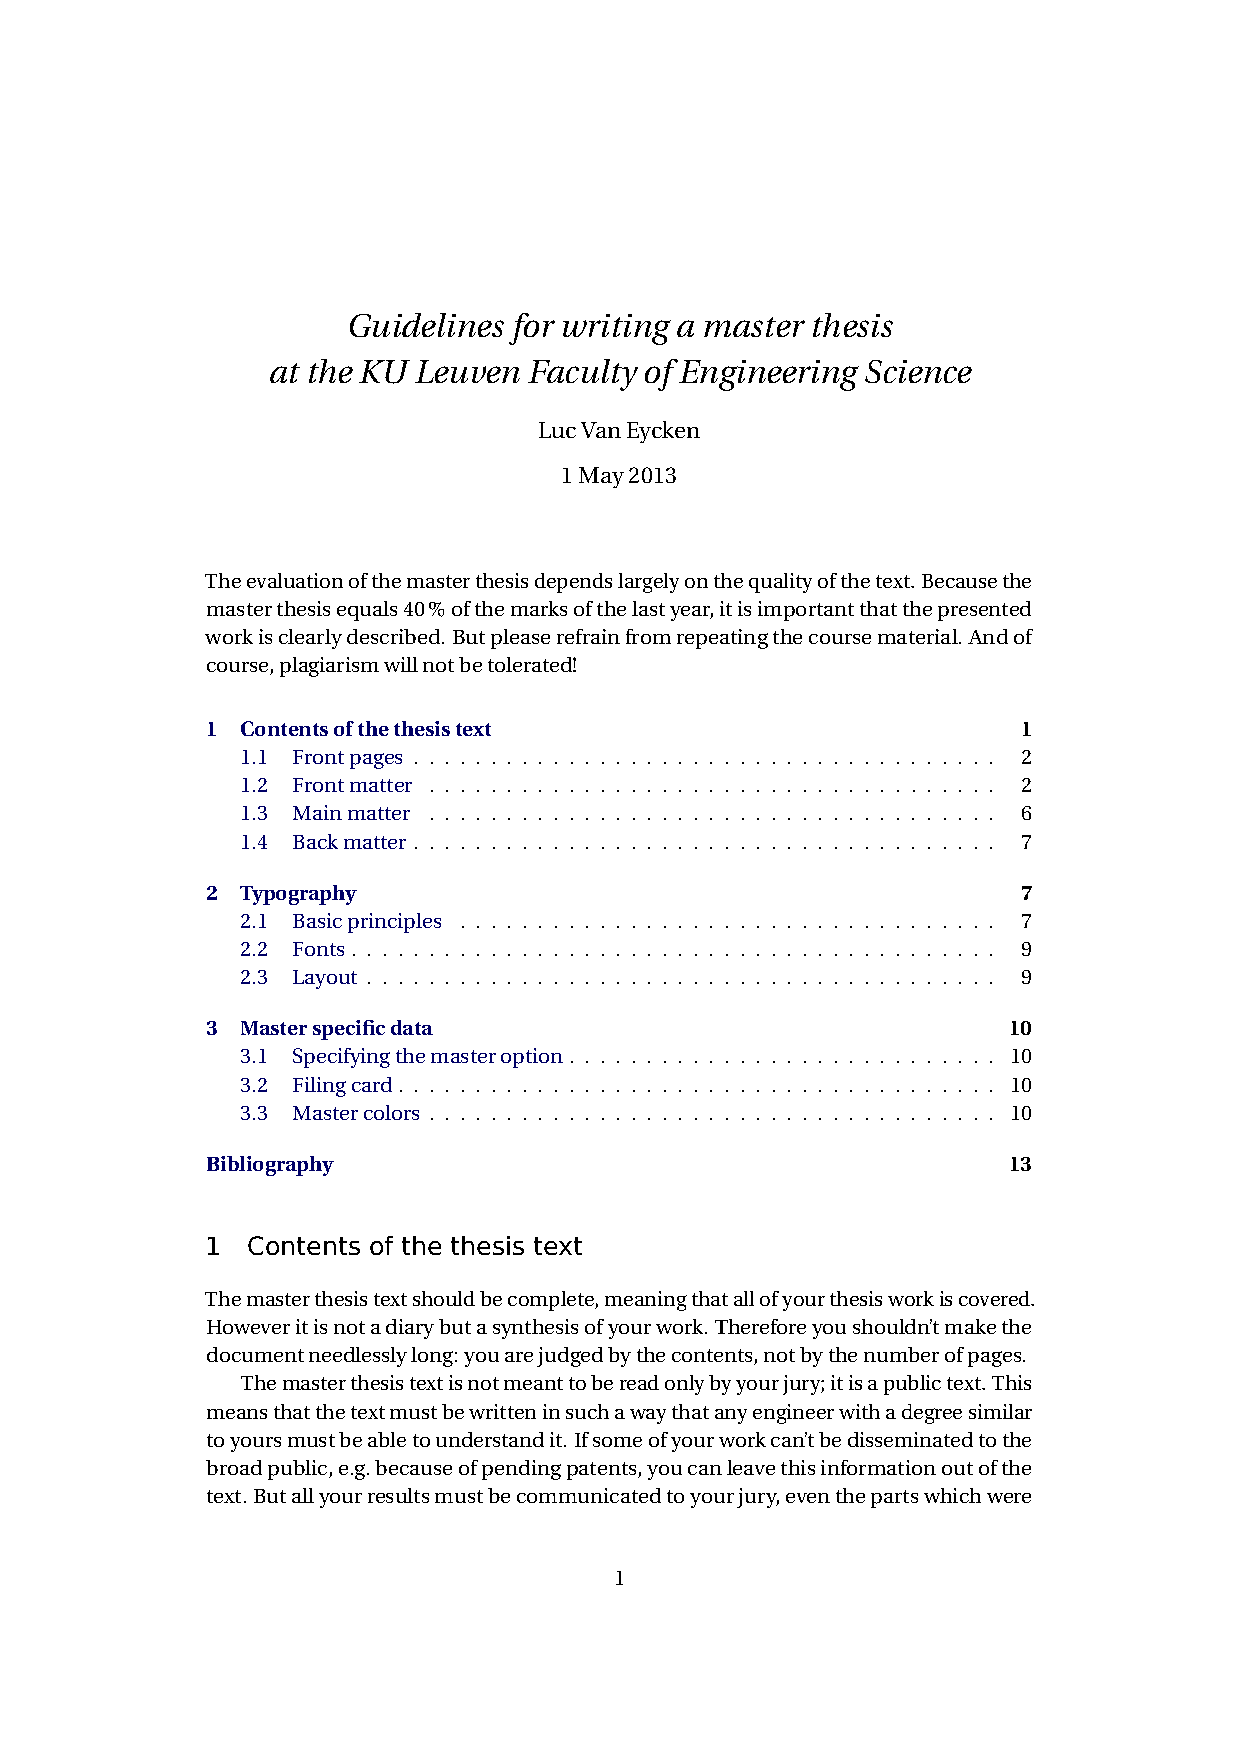
\includepdf[pages=-]{guidelines_thesis.pdf}
%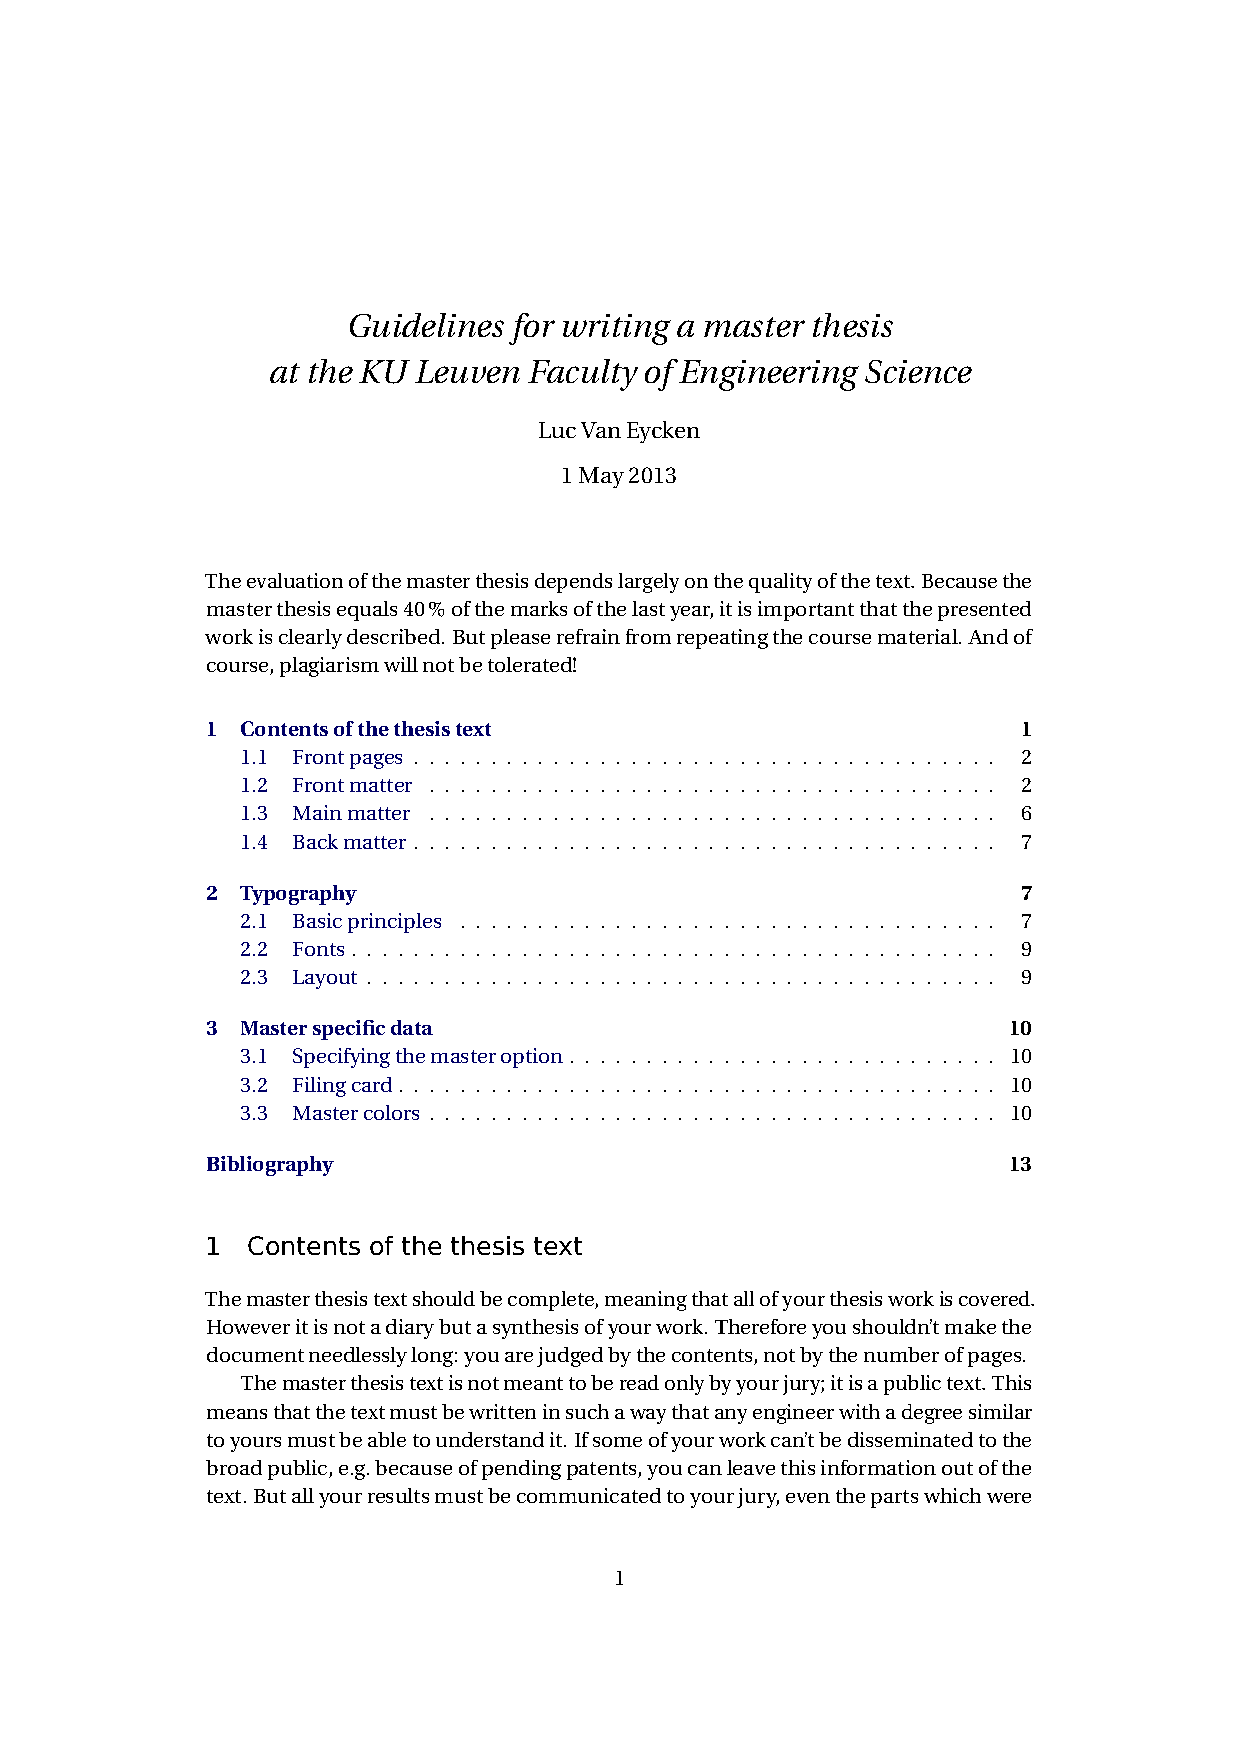
\includepdf[pages={1-2}]{guidelines_thesis.pdf}
%\includepdf[pages=-]{loonjobatprofielvoorbudgetgebruikt.pdf}

%\chapter{bijlage 2}

%\chapter{De eerste bijlage}
\label{app:A}
In de bijlagen vindt men de data terug die nuttig kunnen zijn voor de
lezer, maar die niet essentieel zijn om het betoog in de normale tekst te
kunnen volgen. Voorbeelden hiervan zijn bronbestanden,
configuratie-informatie, langdradige wiskundige afleidingen, enz.

In een bijlage kunnen natuurlijk ook verdere onderverdelingen voorkomen,
evenals figuren en referenties\cite{h2g2}.

\section{Meer lorem}
\lipsum[50]

\subsection{Lorem 15--17}
\lipsum[15-17]

\subsection{Lorem 18--19}
\lipsum[18-19]

\section{Lorem 51}
\lipsum[51]

%%% Local Variables: 
%%% mode: latex
%%% TeX-master: "masterproef"
%%% End: 

% ... en zo verder tot
%\chapter{De laatste bijlage}
\label{app:n}
In de bijlagen vindt men de data terug die nuttig kunnen zijn voor de
lezer, maar die niet essentieel zijn om het betoog in de normale tekst te
kunnen volgen. Voorbeelden hiervan zijn bronbestanden,
configuratie-informatie, langdradige wiskundige afleidingen, enz.

\section{Lorem 20-24}
\lipsum[20-24]

\section{Lorem 25-27}
\lipsum[25-27]

%%% Local Variables: 
%%% mode: latex
%%% TeX-master: "masterproef"
%%% End: 


\backmatter

%for bibtex
% Na de bijlagen plaatst men nog de bibliografie.
% Je kan de  standaard "abbrv" bibliografiestijl vervangen door een andere.
%\nocite{*}
%\bibliographystyle{abbrv}
%\bibliography{referenties}

\chapter{Bibliografie}


%for bibLatex
%\printbibliography[heading=bibintoc,title={Whole bibliography}] %Prints the entire bibliography with the titel "Whole bibliography"

%hiermee worden alle entries getoond, zelfs als ze niet vermeld worden in de tekst.
%\nocite{*}

%Filters bibliography
\printbibliography
\printbibliography[heading=subbibintoc,type=online,title={Sites only}]
\todo[inline]{Gebruikte bronnen en sites nog als bibliografie toevoegen achteraan.}

%\printbibliography[heading=subbibintoc,type=article,title={Articles only}]
%\printbibliography[heading=subbibintoc,type=book,title={Books only}]

%op aparte pagina zo schrijven dan
%\printbibliography[type=book,title={Books only}]
%\printbibliography[keyword={physics},title={Physics-related only}]
%\printbibliography[keyword={latex},title={\LaTeX-related only}]

%\chapter{Index}

\printindex


\end{document}

%%% Local Variables:
%%% mode: latex
%%% TeX-master: t
%%% End:
